\documentclass[10pt]{article}
\usepackage[margin=0.9in]{geometry}
\usepackage[T1]{fontenc}
\usepackage[utf8]{inputenc}
\usepackage{lmodern}
\usepackage{textcomp}
\usepackage{microtype}
\usepackage{booktabs}
\usepackage{array}
\usepackage{graphicx}
\usepackage{listings}
\usepackage{xcolor}
\usepackage{tikz}
\usetikzlibrary{arrows.meta,positioning}
\usepackage[numbers,sort&compress]{natbib}
\usepackage[colorlinks=true,linkcolor=blue!50!black,citecolor=blue!50!black,urlcolor=blue!50!black]{hyperref}

\lstset{
  basicstyle=\ttfamily\footnotesize,
  breaklines=true,
  columns=fullflexible,
  keepspaces=true,
  frame=single,
  framesep=4pt,
  xleftmargin=4pt,
  showstringspaces=false,
  escapeinside={(*@}{@*)},
}

\newcommand{\rt}{Rhylthyme}
\newcommand{\code}[1]{\texttt{#1}}
\newcolumntype{R}[1]{>{\raggedright\arraybackslash}p{#1}}

\title{\rt{}: A Declarative Language and Agent-Native Runtime for\\Human-Executed, Resource-Constrained Schedules}
\author{Jeremy Leipzig\\\texttt{leipzig@gmail.com}}
\date{September 2026}

\begin{document}
\maketitle

\begin{abstract}
Scheduling software tends to fall into three kinds: tools that compute a plan and hand it to a person as a static artifact; engines that execute a dependency graph on machines with no person in the loop; and checklists with timers that walk a person through steps without any model of shared resources or parallel work. \rt{} (``real time'') is built for what falls between them: capacity-constrained, multi-track schedules whose executor is a human working against a clock, with steps the executor starts and ends. We describe (i) a compact JSON language of parallel tracks, timed steps, dependency triggers, environments and resource constraints, annotated with workflow and time ontology terms; (ii) a validator, an auto-planner with several strategies, and two runtimes (a terminal runner and a web player with timeline, itinerary and dependency-graph views); and (iii) a Model Context Protocol server that exposes validation, timing analysis, catalog search, import and publication as annotated tools, so that a language-model agent can author and deliver a schedule as tool calls rather than prose. We position the system as a natural extension of traditional project scheduling techniques, and compare it with air-traffic flow management, temporal constraint networks and robot task scheduling, cooking-step and laboratory schedulers, lab-automation software, and workflow engines, arguing that its contribution is a narrow one: capacity constraints and cross-track dependencies inside a followable, human-executed timeline, one schema used across domains, and an agent interface whose validator refuses malformed programs before they are published.
\end{abstract}

\section{Introduction}

Many tasks consist of several manual steps carried out in serial or in parallel, under resource constraints, with durations that are only partly known in advance. A cook coordinating four dishes so that they finish together, a technician running a protocol whose incubations overlap, a stage manager calling cues, and a trainer running supersets all face the same structure: several sequential lines of work that run at once, dependencies between them, durations that are sometimes fixed and sometimes open-ended, and a handful of resources (one oven, two thermocyclers, one PA system) that cannot be used by more than a bounded number of steps at a time. Abbott, Bogart and Walkingshaw call the artifacts that describe such work ``programs for people'': recipes, protocols and run sheets are written by one person to be executed by another, present an idealized linear process, and rely on conventions for widening or narrowing what a step means~\cite{abbott2015programs}.

Computers have offered solutions to these logistical timing problems for decades. The Gantt chart, a bar chart with one row per activity and time on the horizontal axis; the critical path method (CPM), which links activities by precedence and finds the chain that determines the finish date; the Program Evaluation and Review Technique (PERT), which does the same with three duration estimates per activity (optimistic, most likely, pessimistic) so that the finish date carries an uncertainty; and resource-constrained project scheduling, which adds limited resources that activities compete for, all produce a plan from a formal description of the work~\cite{wilson2003gantt,kelley1959cpm,malcolm1959pert,brucker1999rcpsp}. The obstacle has been the description. Representing a schedule in a machine-readable syntax is too arduous for the people who actually run these tasks, and mixed-initiative scheduling workbenches, which tried to meet users halfway with interactive editing of a formal model, never reached the kitchen or the bench~\cite{hsu1993macmerl,norbis1996interactive}. Before large language models, an end user had no way to state a schedule, its constraints, or how it should be optimized in natural language and have software act on the statement. That has changed: language-model agents now translate free-text protocols into executable form and draft formal planning problems from prose~\cite{shi2024protocol,angelopoulos2026prompts,benyamin2025copilot}, which makes a compact, well-specified target syntax worth having.

Meanwhile, the systems that do handle logistics in real time fall at the extremes. Some are highly specialized and proprietary: airline operations and air-traffic flow management run on bespoke optimization and collaborative decision-making platforms~\cite{bertsimas1998atfm,wambsganss1996cdm}. Some are entirely manual: a bench laboratory typically runs overlapping incubations with an array of kitchen timers and sticky notes, and the protocol platforms that assist it step through a checklist with a single timer~\cite{teytelman2016protocolsio}. And some are entirely automated: factory scheduling, liquid-handling robots and self-driving laboratories dispatch steps to machines that need no explanation~\cite{wierenga2023pylabrobot,opentronsapi,tom2024sdl}. Between the extremes, the tooling that does put a person in the loop (guided-cooking timers, show control, protocol run modes) lacks the project-scheduling model of parallel tracks, cross-track dependencies and capacity limits on shared resources, while domain schedulers for kitchens and laboratories have the model but stop at an optimized procedure~\cite{matsushima2015cooking,nakabe2021cooking,zhou2026sdlscheduling}. Workflow engines and laboratory orchestrators execute dependency graphs, but their executors are compute nodes, robots or instruments, and their objective is reproducible output rather than a followable timeline~\cite{leipzig2017pipelines,tom2024sdl}.

\rt{} is a small system built for the intersection. Its contributions are:

\begin{enumerate}
  \item \textbf{A language.} A JSON program model of parallel \emph{tracks} of sequential \emph{steps}, with a fixed vocabulary of start triggers, three kinds of duration, buffers, choice branches, replicates with staggered starts, and a separate \emph{environment} document that declares resource capacities and the people available to attend them. The schema annotates its constructs with workflow and time ontology terms, so that each has a stated meaning in a standard temporal model.
  \item \textbf{A runtime.} A validator that catches structural and scheduling errors, an auto-planner with named strategies (finish together, minimize length, provide consistent activity coverage, fit to a target time) and over-utilization detection, a curses runner with manual and indefinite steps, actor accounting and abort handling, and a web application whose timeline, itinerary and dependency-graph views play the schedule.
  \item \textbf{An agent interface.} A Model Context Protocol (MCP) server that exposes \code{validate\_program}, \code{analyze\_schedule}, \code{visualize\_schedule}, import from external recipe and protocol sources, catalog search and account tools, with tool annotations, structured output, resources and a prompt. One implementation serves five endpoints (generic, kitchen, laboratory, events, gym) from one schema.
\end{enumerate}

\section{Related work}

\subsection{Gantt charts, CPM and PERT}
The Gantt chart is a century old and, as Wilson notes, its origins are murkier than its ubiquity suggests~\cite{wilson2003gantt}. It remains the dominant visual grammar for ``which activity runs when on which row,'' and \rt{}'s primary view is a Gantt chart whose rows are tracks. CPM~\cite{kelley1959cpm} and PERT~\cite{malcolm1959pert}, both published in 1959, added precedence networks and earliest and latest start times; PERT, built for the US Navy's Polaris programme, assumed each activity's duration follows a beta distribution summarized by its three estimates. \rt{}'s variable durations (\code{minSeconds}, \code{defaultSeconds}, \code{maxSeconds}) are a three-point estimate without PERT's distributional assumptions, and its \code{analyze\_schedule} tool reports the dependency chain that determines the makespan, a critical-chain heuristic rather than CPM's float-based criticality (Section~\ref{sec:runtime}).

\subsection{Resource-constrained project scheduling}
The resource-constrained project scheduling problem (RCPSP) generalizes CPM with renewable resources of bounded capacity; Brucker et al.\ give the standard notation and classification~\cite{brucker1999rcpsp}, Kolisch and Padman survey exact and heuristic methods~\cite{kolisch2001survey}, and Pinedo's textbook is the standard reference for the machine-scheduling models, and the job-shop and flow-shop vocabulary, that these problems extend~\cite{pinedo2016scheduling}. In those terms a \rt{} track is a resource of capacity one (one pair of hands at one station: steps in a track may not overlap, and the validator rejects programs where they do) and each resource constraint is a renewable resource with capacity \code{maxConcurrent}. The difference is in what is done with the model: RCPSP solvers minimize makespan or net present value; \rt{} checks feasibility, surfaces conflict windows, and applies staggering heuristics, leaving the final timing to the person running it.

That division of labour has its own tradition. Mixed-initiative scheduling systems of the 1990s paired a generative scheduler and constraint checker with a manual scheduler and critic so that a person and a program could revise one schedule together~\cite{hsu1993macmerl}; interactive decision-support systems for the resource-constrained scheduling problem let the decision maker change job priorities and priority rules and re-run the heuristic~\cite{norbis1996interactive}; and the rescheduling literature argued early that practical scheduling is a reactive process in which circumstances continually force revision, so reactivity should be a design centre rather than an afterthought~\cite{kelleher1997rescheduling}. \rt{} inherits the manual-editing half of that tradition (the web editor and the auto-planner strategies) and the visualization half (Section~\ref{sec:views}), but not the reactive half: it propagates delays along dependency chains at run time and does nothing more (Section~\ref{sec:runtime}). Timing also matters on the human side of the loop: Yu et al.\ show experimentally that the rhythm at which a mixed-initiative system takes and yields the initiative affects users' sense of agency, performance and stress~\cite{yu2017timing}, which bears directly on how a runtime should fire audio cues and present manual gates.

\subsection{Real-time flow management in air traffic control}
Air-traffic flow management is the archetype of scheduling that is both resource-constrained and continuously replanned. Bertsimas and Stock Patterson formulate it as an integer program over airport and sector capacities and show it is NP-hard~\cite{bertsimas1998atfm}; Ball et al.\ give a stochastic ground-holding model designed to integrate with Collaborative Decision Making (CDM)~\cite{ball2003groundholding}, the FAA/airline information-sharing regime of the 1990s~\cite{wambsganss1996cdm}. Two ideas transfer, at a very different scale. Capacity is a cap on concurrent occupancy of a shared resource over a time window, which is \rt{}'s \code{maxConcurrent}; and CDM's premise that the plan is a shared artifact updated as participants act is the premise of \rt{}'s shareable timeline, though \rt{} has no optimization layer and does not yet merge progress across participants.

\subsection{Temporal reasoning and robot task scheduling}
\rt{}'s triggers are temporal constraints between intervals. Allen's interval algebra~\cite{allen1983intervals} names the qualitative relations and OWL-Time gives them a web vocabulary~\cite{hobbs2004owltime,w3c2020owltime}; the \rt{} schema uses that vocabulary to annotate its constructs (Section~\ref{sec:ontology}). Dechter, Meiri and Pearl's temporal constraint networks~\cite{dechter1991tcn} add metric bounds; a \rt{} program restricted to fixed durations, non-negative offsets and conjunctive triggers is a simple temporal network whose consistency the validator checks by resolving all start times. Temporal networks with uncertainty~\cite{vidal1999stnu,morris2001dc} model durations the executor does not control; \rt{}'s variable and indefinite steps are the other case, durations the executor \emph{does} control by ending the step, and we return to the distinction in Section~\ref{sec:limits}.

Robotics contributes the allocation side. Gerkey and Matari\'c's taxonomy of multi-robot task allocation~\cite{gerkey2004mrta} and its extension to interrelated utilities and constraints by Korsah et al.~\cite{korsah2013mrta} classify who does what; Gombolay, Wilcox and Shah's Tercio schedules human--robot teams under tight temporospatial constraints with a satisficing sequencer inspired by real-time processor scheduling~\cite{gombolay2018tercio}. \rt{}'s environments express the same allocation constraints declaratively (actor types with counts, per-task attention requirements and qualifications), but the runtime only accounts for them; it does not solve an assignment problem. Behavior trees~\cite{colledanchise2018bt} are the reactive-execution counterpart: like \rt{}'s runner they execute a declarative structure tick by tick and react to manual and abort events, but they are control-flow trees rather than timed parallel tracks.

\subsection{Domain schedulers: kitchens and laboratories}
Cooking several dishes at once has been treated as a scheduling problem for decades. Guley and Stinson solved food-service production scheduling by branch and bound in 1984~\cite{guley1984foodservice}, and scheduling several recipes onto one timeline in front of the cook dates to Cooking Navi, which reads recipe text into a cooking workflow and reorders the steps of several dishes into one presented sequence~\cite{hamada2005cookingnavi}; the kitchen HCI work of the same period was already showing the cook what had just been done, in Cook's Collage's replay of the last few actions~\cite{tran2005collage}. Matsushima and Funabiki decompose recipes into six cooking-step types, schedule them under cook and utensil constraints, and present the result through a guidance interface~\cite{matsushima2015cooking}; Nakabe et al.\ build a task graph per recipe and present an optimal parallel procedure~\cite{nakabe2021cooking}. These are the closest prior systems to \rt{}'s kitchen vertical. They differ in that each computes a procedure and presents it once, whereas \rt{} keeps the resource model live during execution, with a clock, cues, manual steps, and the ability to save, share and re-run.

On the laboratory side, workflows that mix wet-lab and digital tasks were being reasoned about, for cost, quality and ordering, before the current wave of automation~\cite{lacroix2009workflows}. Self-driving laboratories (SDLs) have since made scheduling a first-class concern. Tom et al.\ survey the field~\cite{tom2024sdl}; the HELAO framework orchestrates distributed instruments running parallel, asynchronous experiments with device sharing and provenance~\cite{rahmanian2022helao}; Zhou et al.\ formulate multi-task SDL scheduling with operation precedence, station allocation and time-synchronization constraints under which one operation must begin the instant its predecessor ends~\cite{zhou2026sdlscheduling}; the Artificial platform orchestrates whole-lab workflows, including manual steps performed by scientists~\cite{fehlis2025artificial}. Closer to genomics, Arteria automates the data side of sequencing core facilities in three layers (event-based orchestration, processes modelled as workflows, and execution by RESTful micro-services) and has been deployed at three facilities~\cite{dahlberg2019arteria}; its events drive data processing rather than bench work, but it shares \rt{}'s separation of a process description from the runtime that advances it. Two recent lines of work sit closest to \rt{}'s import and authoring paths: Shi et al.\ translate human-readable protocols into machine-interpretable protocol dependence graphs while preserving causality and consistency~\cite{shi2024protocol}, and Angelopoulos et al.\ give an orchestration system an LLM agent that creates and monitors protocols from natural language, with automated validation and error correction and the ability to alternate between agent-assisted and manual construction~\cite{angelopoulos2026prompts}. Both target robotic execution; the same moves (structured translation, validate-and-correct authoring) are what \rt{} applies to protocols a person will run. Beneath the schedulers sits a layered software landscape: device-level standards and drivers (SiLA~2's typed feature definitions over gRPC~\cite{sila2}, the Opentrons Python Protocol API~\cite{opentronsapi}, PyLabRobot's hardware-agnostic liquid-handling interface~\cite{wierenga2023pylabrobot}); a machine-readable protocol layer (Autoprotocol's JSON protocol description~\cite{autoprotocol}, BioCoder's typed language for writing biology protocols so that they can be standardized and automated~\cite{ananthanarayanan2010biocoder}, and the chemical programming language that drives a modular robotic synthesizer~\cite{steiner2019chemputer}); and a human-readable protocol layer (protocols.io, whose run mode already gives a scientist a checklist with a timer~\cite{teytelman2016protocolsio}, and electronic notebooks such as Benchling). Aquarium spans the two: a protocol is a program the laboratory executes, but the executing agent is a technician the software instructs step by step while it tracks samples and data~\cite{vrana2021aquarium}. \rt{} sits at the human end of this stack but imports from both ends: it converts protocols.io and Benchling protocols \emph{and} Opentrons protocol scripts into timed, resource-aware programs a bench scientist runs by hand, and its \code{afterStep} trigger with zero offset is the human-executed analogue of the SDL synchronization constraint.

\subsection{Workflow engines and process notations}
Configuration-based bioinformatics pipeline frameworks are the closest \emph{architectural} relatives: a declarative description of steps and dependencies, a validator, an execution engine and a set of importers. We previously surveyed these frameworks along three axes: implicit versus explicit syntax, configuration/convention/class design paradigm, and command-line versus workbench interface~\cite{leipzig2017pipelines}. On those axes \rt{} is an explicit-syntax, configuration-paradigm system offered through both a command line and a web workbench. What separates it from the frameworks is not architecture but executor and objective: pipeline engines run on machines and optimize for reproducible output across compute environments, and some now expose their platforms to agents through vendor MCP servers; \rt{} runs on a person and optimizes for a timeline that can be followed. The same contrast holds against the newest member of the family, an MCP-native workflow engine in which an agent reasons once to produce a declarative JSON blueprint of tool calls, with loops, parallel branches and data piping, that is then executed without further reasoning~\cite{parmar2026mcpworkflow}: a \rt{} program is also a declarative JSON document produced by an agent, but its steps are executed by a person at the stove or the bench, not by the engine. Closest in form is McKeever et al.'s scheduler, which defines a platform-agnostic JSON representation of workflows that keeps execution details apart from the scientific logic, translates Nextflow workflows into it through an executor plugin, and puts a graphical interface in front of it for non-technical users~\cite{mckeever2025scheduler}. The parallel with \rt{}'s schema, importers and web editor is close; the difference, again, is the executor: SLURM-managed HPC nodes rather than a person. The nearest analogue in the human-process world is BPMN~2.0~\cite{omg2011bpmn}, whose execution semantics include user tasks assigned to people and timer events; BPMN models control flow, roles and messages, and leaves capacity limits on shared resources and the wall-clock playback of a schedule to the engine that hosts it.

\section{The \rt{} program model}
\label{sec:model}

A \rt{} program is a JSON document validated against a JSON Schema (version 0.2.0-alpha at the time of writing). Figure~\ref{fig:thanksgiving} shows a five-track Thanksgiving dinner planned around one oven, rendered by the bundled timeline renderer; Listing~\ref{lst:step} shows three of its steps. Table~\ref{tab:concepts} defines the concepts the language shares with every schedule of this kind, with one example from each vertical.

\begin{figure}[t]
  \centering
  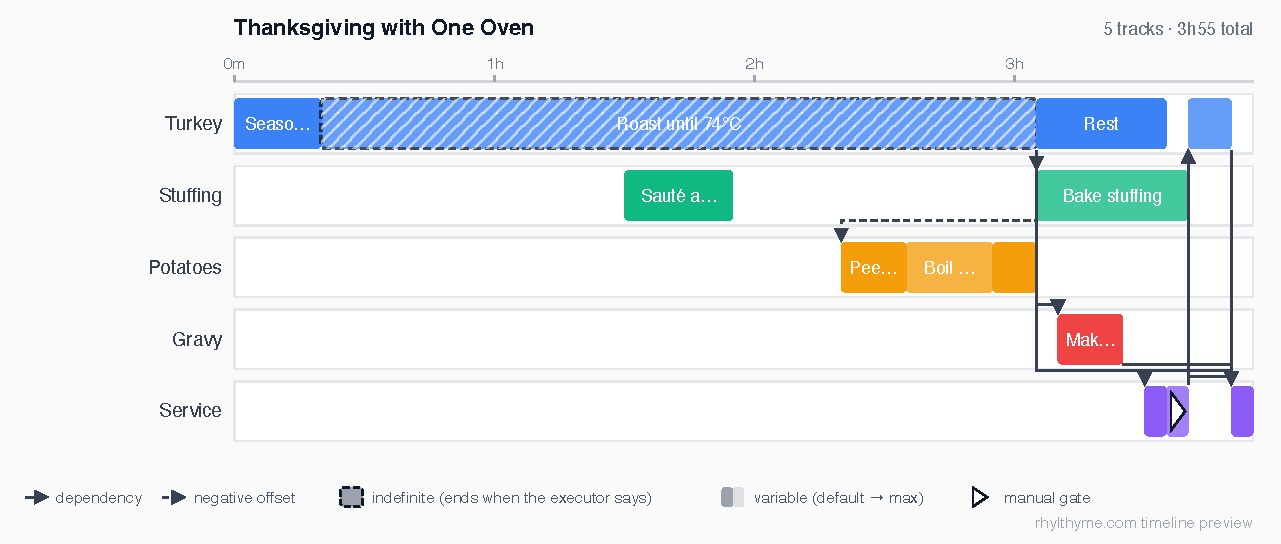
\includegraphics[width=\linewidth]{figures/thanksgiving-gantt.pdf}
  \caption{\emph{Thanksgiving with One Oven} (five tracks, thirteen steps, 3\,h\,55 at planned durations) as rendered by the open-source timeline renderer (\code{@rhylthyme/timeline}) that also produces the MCP server's image previews. Rows are tracks; bars are steps positioned by resolved start time. The roast is \emph{indefinite} (hatched, dashed border): it ends when the cook says so, and everything downstream is planned against its default duration. Arrows are cross-track dependencies; the dashed arrow is a negative offset (peel the potatoes 45\,min before the roast is due out). The flag on ``Guests seated'' marks a \emph{manual} gate that the host fires; ``Carve'' waits for it, and ``Serve'' waits for all four dishes. The oven is a capacity-one resource, so the stuffing bakes only after the turkey comes out. The web application draws its own D3 timeline from the same JSON.}
  \label{fig:thanksgiving}
\end{figure}

\begin{lstlisting}[caption={Three steps from Figure~\ref{fig:thanksgiving}: an indefinite roast that occupies the oven until the cook ends it; a step that starts 45 minutes before the roast is due to end; and a manual gate that the host fires when guests sit down.},label={lst:step}]
{ "stepId": "turkey-roast", "name": "Roast until 74(*@\textdegree@*)C", "task": "oven",
  "duration": { "type": "indefinite", "defaultSeconds": 9900 },
  "startTrigger": { "type": "afterStep", "stepId": "turkey-prep" } },
{ "stepId": "potatoes-peel", "name": "Peel and cut", "task": "prep",
  "duration": { "type": "fixed", "seconds": 900 },
  "startTrigger": { "type": "afterStep", "stepId": "turkey-roast",
                    "offsetSeconds": -2700 } },
{ "stepId": "guests-seated", "name": "Guests seated", "task": "host",
  "duration": { "type": "fixed", "seconds": 300 },
  "startTrigger": { "type": "manual", "triggerName": "guests-seated" } }
\end{lstlisting}

\begin{table}[t]
  \centering\footnotesize
  \setlength{\tabcolsep}{4pt}
  \begin{tabular}{@{}R{2.2cm}R{5.6cm}R{8.6cm}@{}}
    \toprule
    Concept & Definition (\rt{} construct) & Examples \\
    \midrule
    Program & The whole schedule: a named set of tracks plus its resources and metadata (\code{programId}, \code{tracks}, \code{resourceConstraints}) & Thanksgiving dinner; a Western blot; a wedding run-of-show; a 45-minute HIIT session \\
    Track & One line of work whose steps run one after another; parallel work goes in separate tracks & The turkey; the gel; the ceremony; the lower-body superset \\
    Step & A single timed activity within a track (\code{stepId}, \code{duration}, \code{task}) & Roast 3\,h; incubate 1\,h; procession 5\,min; 12 reps \\
    Dependency & A condition on when a step may start, within or across tracks (\code{startTrigger}: after a step ends or starts, at an offset from program start, on a manual signal, on abort, or all/any of several) & Gravy starts when the turkey comes out; blocking starts after transfer; music cue fires when the doors open; rest starts after the last set \\
    Offset & A signed delay applied to a dependency; negative offsets start a step before its anchor ends & Potatoes in 20\,min before the roast finishes; pre-warm the reader 10\,min before the plate is ready \\
    Buffer & Setup or cleanup time attached to a step, or an explicit gap between two steps (\code{preBuffer}, \code{postBuffer}, \code{afterStepWithBuffer}) & Preheat before baking; centrifuge spin-down; stage reset between acts; equipment changeover \\
    Fixed / variable / indefinite duration & Exact time; bounded time the executor may end early; open-ended time the executor ends & Bake 25\,min; saut\'e 3--5\,min; incubate overnight until confluent; hold until the speaker finishes \\
    Resource and capacity & A named task type with a limit on concurrent use (\code{task}, \code{maxConcurrent}) & One oven; two thermocyclers; one PA system; one squat rack \\
    Actor and attention & People available to attend steps, by type and count, and the fraction of a person each resource needs (\code{actorTypes}, \code{actorsRequired}, \code{qualifiedActorTypes}) & A stove burner needs one cook; a microwave a quarter of one; only a licensed operator runs the cytometer \\
    Environment & A reusable document declaring the resources and actors of a workplace, referenced by programs (\code{environment}) & Home kitchen with two cooks; small academic lab; theater; gym floor \\
    Choice & A decision point whose options gate downstream steps (\code{choice}, \code{choiceId}) & Chicken or tofu; run the optional wash; rain plan; beginner or advanced set \\
    Replicate and stagger & The same track or step repeated $n$ times, in parallel, staggered by a delay, or serially (\code{replicates}, \code{batch\_size}, \code{stagger}) & Three trays of cookies 10\,min apart; twelve samples; three landings on one runway \\
    Priority and flex & Ordering for planners when something must give, and permission for a step to stretch to fill a gap (\code{priority}, \code{flex}) & Drop the garnish before the main; let the rest interval fill the gap \\
    Makespan, slack, critical chain & Total resolved time; how early a track finishes; the dependency chain that determines the end & Dinner is 4\,h\,40; the toast track has 6\,min to spare; the turkey chain sets the finish \\
    Manual gate and abort path & A step that waits for the executor's signal; steps that run only if another is aborted (\code{manual}, \code{onAbort}) & ``Start when guests are seated''; discard and re-plate if contaminated \\
    \bottomrule
  \end{tabular}
  \caption{Concepts common to human-executed schedules and how \rt{} expresses them.}
  \label{tab:concepts}
\end{table}

\paragraph{Tracks, steps and triggers.} A program has a \code{programId}, \code{name}, optional \code{environmentType}, optional \code{actors} or an \code{environment} reference, an array of \code{tracks}, optional \code{resourceConstraints} and free-form \code{metadata} (ingredients, serves, source attribution, thumbnail). A track is a named sequence of steps that must not overlap in time; the array order of steps is not itself enforced, only non-overlap. Step identifiers are unique across the whole program so that any step may reference any other. A start trigger is one of \code{programStart}, \code{programStartOffset}, \code{afterStep} (anchored to the referenced step's end, or its start with \code{event:\,start}, plus a signed \code{offsetSeconds}), \code{afterStepWithBuffer}, \code{manual} and \code{onAbort}, or a compound \code{\{logic: all|any, triggers: [\ldots]\}} that waits for all, or the first, of several. Offsets and durations accept a number of seconds or a unit string (\code{"5m"}, \code{"1h30m"}). A trigger may carry a \code{choiceId}; a step with a \code{choice} block presents options at run time, and downstream steps gated on a \code{choiceId} run only for that option. A negative \code{afterStep} offset (``start 20 minutes before the roast is done'') is accepted only against an indefinite step; planners place it against the referenced step's \code{defaultSeconds}, and the runtimes fire it from that forecast rather than from the actual end, a limitation discussed in Section~\ref{sec:limits}.

\paragraph{Durations.} A \emph{fixed} duration has \code{seconds}. A \emph{variable} duration has \code{minSeconds} and \code{maxSeconds}, an optional \code{defaultSeconds} used for planning, and may be ended early by the executor. An \emph{indefinite} duration runs until the executor ends it; \code{defaultSeconds} gives planners something to draw. In every case the person running the program decides when a non-fixed step ends; the language has no construct for a duration that is uncertain \emph{and} outside the executor's control.

\paragraph{Environments.}
\label{sec:environments}
An environment is a separate JSON document, validated against its own schema, that describes a workplace once so that many programs can share it. It has an \code{environmentId}, a \code{type} from a controlled list (37 values, from \code{kitchen} and \code{laboratory} to \code{theater}, \code{gym} and \code{datacenter}), \code{actorTypes} (named categories of people with a \code{count}), and \code{resourceConstraints}. Each constraint names a task, its \code{maxConcurrent} capacity, the fraction of a person it occupies (\code{actorsRequired}: an oven needs 0.5 of a cook, a microwave 0.25, a stove burner 1.0), and which actor types are \code{qualifiedActorTypes} for it. A program references an environment by id; the loader falls back to the default environment for the program's \code{environmentType} when none is named, and inline \code{resourceConstraints} on the program take precedence. The repository ships ten environments (home and commercial kitchens, academic, biotech and pharma laboratories, a bakery, an airport, a software team), and \code{create\_environment} on the MCP server produces new ones. A program that names neither an environment nor \code{actors} must declare a resource constraint for every task it uses. Environments are what let the same protocol be scheduled differently in a lab with one thermocycler and a lab with four; the attention and qualification fields are honoured by the command-line runner, while the web and MCP engines use only capacities and the program-level actor count.

\paragraph{Replicates and staggered starts.}
Repetition has a shorthand so that authors need not copy tracks. A track may declare \code{batch\_size} and \code{stagger}: \code{"batch\_size": 3, "stagger": "1m30s"} expands into three copies of the track whose starts are 90 seconds apart, and \code{templateId} with \code{templateParameters} lets those copies instantiate a shared \code{trackTemplates} entry with different values (three landings on one runway with different flight numbers, in the airport example). A track or step may instead declare \code{replicates} with a \code{count}, a \code{mode} of \code{parallel}, \code{stagger} or \code{serial}, and a \code{delay}; step-level parallel replicates fan out into sub-tracks that rejoin, serial replicates chain within the track, and staggered replicates delay each start by the given amount. Expansion happens before validation in both toolchains, so the validators, planners and runtimes only ever see plain tracks and steps.

Schema 0.3.0-alpha adds three constructs that say what happens \emph{downstream} of a replicated step, per instance. A step-referencing trigger may carry \code{instances}: \code{"each"} replicates the dependent step once per instance and pairs instance $i$ with instance $i$ of its predecessor (each tray of cookies starts cooling the moment it leaves the oven), \code{"all"} is a barrier that waits for every instance, and \code{"any"} fires on the first --- the multiple-instance, synchronization and discriminator patterns of the workflow-pattern catalogue~\cite{vanderaalst2003patterns}, written on a trigger rather than drawn in a graph. The default is \code{"all"}, which is the rejoin that earlier schema versions already performed, so existing programs keep their timings. A replicated step may also declare \code{maxInFlight}: a bound on how many instances may be \emph{in flight} between it and its barrier, where an instance is in flight from its own start until it has finished every \code{"each"} descendant. This is not \code{maxConcurrent}, which bounds occupancy of one task at one instant; \code{maxInFlight} bounds a chain of tasks across time, and the difference is operational rather than cosmetic. A cooling rack that holds two trays, declared as \code{maxConcurrent: 2}, would let a third tray bake and then leave it hot with nowhere to go; declared as \code{maxInFlight: 2} it holds the third \emph{bake} until a tray leaves the rack. Hold the upstream step, do not strand the downstream one. The same shape is a centrifuge rotor that holds six tubes, a bench with room for four open plates, or a taxiway between landing and gate. The three constructs are McKeever et al.'s asynchronous nodes, barrier nodes and maximum asynchronous concurrency~\cite{mckeever2025scheduler}, carried over from compute workflows, where the bounded resource is disk space, to human-executed schedules, where it is oven racks, rotors and bench space. Expansion rewrites all three into plain \code{afterStep} and \code{compound} triggers, the same reduction of higher-level routing constructs to a small primitive set on which Petri-net workflow semantics rest~\cite{vanderaalst1998petri} --- the in-flight bound becomes a synthetic conjunction on instance $i + k$ that also waits for the last descendant of instance $i$ --- so the addition costs the validators, planners and runtimes nothing beyond the expander pass, and because \code{afterStep} fires on actual completion, a tray that cools slowly really does hold up the next bake.

\section{Ontologies and vocabularies}
\label{sec:ontology}

The program and environment schemas carry \code{\$comment} annotations written in the vocabulary of the W3C Time Ontology in OWL~\cite{hobbs2004owltime,w3c2020owltime}, itself grounded in Allen's interval relations~\cite{allen1983intervals}. A step is a \code{time:ProperInterval} with a \code{time:hasBeginning} and \code{time:hasEnd}; a fixed duration is a \code{time:Duration} with \code{time:numericDuration} in \code{time:unitSecond}; \code{afterStep} with zero offset is \code{time:intervalMetBy} and with a positive offset \code{time:intervalAfter}; a pre-buffer \code{time:intervalMeets} its step and a post-buffer is \code{time:intervalMetBy} it; \code{programStartOffset} places a \code{time:Instant} relative to program start; compound triggers are conjunctions or disjunctions of these relations. The annotations are documentation, not an RDF export: they fix the intended meaning of each construct for implementers of the validator, the two runtimes and the renderer, and they make the mapping to the temporal-reasoning literature explicit rather than folkloric. Generating OWL-Time individuals from a program is a small transformation we have not built. A second mapping, to provenance rather than time, is just as direct: a step is a PROV-DM \code{Activity}, a resource an \code{Entity} and an actor an \code{Agent}~\cite{moreau2013provdm}, which is the vocabulary in which a run record would be exported. A more ambitious use of the same annotations would compile them into the tool interface itself, so that an agent could only construct programs that satisfy the ontology's constraints; Zhou et al.\ demonstrate that ontology-to-tools compilation for LLM agents on a knowledge-graph platform~\cite{zhou2026ontology}. \rt{} enforces its constraints after generation, through the validator, rather than during it.

Three smaller controlled vocabularies do practical work. The environment \code{type} list names the kinds of workplace the system knows how to default. An instrument catalog groups laboratory and kitchen equipment into categories (centrifuges, thermal cyclers, plate readers, liquid handling, cold storage, ovens, ranges, mixers, proofers, and so on) with default capacities and attention requirements, so that an environment can be assembled by picking instruments. And the public recipe catalog --- an imported corpus far smaller than the recipe datasets assembled for text generation~\cite{bien2020recipenlg} --- is faceted by a fixed taxonomy of categories, cuisines, diets, time buckets, main ingredients, methods and tags, which the search API validates strictly so that a mistyped facet fails loudly rather than silently returning nothing.

\section{Runtime and tooling}
\label{sec:runtime}

\paragraph{Validation.} There are two validators. The Python one, used by the command-line tools, runs JSON Schema validation and then logic checks: duplicate or missing identifiers, references to non-existent steps, choice references to options that do not exist, tasks without a resource constraint, and, after resolving every start time, steps that overlap within a track. The JavaScript one, used by the MCP server, performs the same logic checks without the schema pass, adds dependency-cycle and unparseable-duration detection, and reports each finding with a stable code, a message and a \emph{fix} hint (``chain \code{s2} with \code{\{type:\,afterStep, stepId:\,s1\}} or move it to its own track''), which matters when the author is a language model that will act on the message verbatim. The two share one timing semantics: a parity test resolves every program in the example corpus with both and asserts identical start and end times, currently 616 steps across 39 programs. The top-level corpus holds 38 JSON programs (15 kitchen, 6 laboratory, 4 event, 3 fitness, 2 bakery, 2 airport, 1 manufacturing, 5 general or test); both validators reject the same three, two for within-track overlaps and one for tasks with no resource constraint.

\paragraph{Common optimizations.}
\label{sec:optim}
The auto-planner, available from the web editor and as a Python module, works from earliest start times under the dependency graph, checks the result for resource over-utilization (intervals where more steps occupy a task than its capacity allows), and offers four named strategies that correspond to what people actually ask a schedule to do: \emph{synchronized finish} delays shorter tracks so that every track ends at the same moment (dinner on the table together); \emph{minimize length} packs steps as early as dependencies allow; \emph{provide consistent activity coverage} sequences steps one after another, alternating tracks, so that a single executor always has something to do and no long idle gaps open up; and \emph{fit to time} compresses flexible steps and omits low-priority ones until the program meets a target duration, using each step's \code{priority} and \code{flex} settings (a flexible step may \code{fill} the gap to its successor or stretch to its \code{maxDuration}). All four are heuristics over earliest-start times and dependency order, not solvers; they report over-utilization rather than resolving it, and their job is to hand the person a feasible schedule and to say where the pressure is. (An older planner in the core library predates the current schema and is not described here.)

\paragraph{Analysis.} \code{analyze\_schedule} resolves all start times and computes the makespan; the chain of predecessors that determines it (walking back from the last-ending step through the predecessor whose end is closest to each start); resource-conflict windows by a sweep line over each task's occupancy; peak concurrency against declared actors; per-track slack before the program's end; and, given a \code{finishAt} or \code{startAt} instant, the wall-clock start of every step. ``When do I put the potatoes in so that everything is ready at six'' is a single call. Each conflict window is tagged with the \code{kind} of limit it violates, \code{maxConcurrent} or \code{inFlight}, and a \code{bindingConstraints} list names, for every edge of the critical chain, which limit actually gates it: for the three-tray example above the analyzer reports the rack rather than the oven, which is the answer the cook needs.

\paragraph{Execution.} Two runtimes play a program. The command-line runner is a curses interface that advances a clock, starts steps as their triggers fire, waits on manual triggers, lets the executor end variable and indefinite steps, accounts for actor capacity from the environment, and handles abort with \code{onAbort} triggers. Because \code{afterStep} triggers fire on actual completion, a step that runs long delays everything chained after it, while steps anchored to program start by offset stay on the clock; there is no replanning beyond that propagation. The web application is a player: it advances a simulated clock on a browser interval timer at a chosen speed, starts and highlights steps as their resolved times arrive, and lets the executor end non-fixed steps; it is not re-anchored to wall-clock time while running, so a phone that sleeps mid-roast pauses the schedule rather than catching up. It renders the program in three principal views and several auxiliary ones (Section~\ref{sec:views}). Both runtimes consume the same JSON, and both are what the MCP server links to.

\paragraph{Importers.} A registry of importers, plus a separately authenticated Benchling connector, converts external sources into programs: Spoonacular and TheMealDB recipes, Cooklang files, protocols.io and Benchling protocols, and Opentrons Protocol API scripts. Importers infer tracks and durations from source structure, a much weaker form of the protocol-to-dependence-graph translation that Shi et al.\ pursue for robotic labs~\cite{shi2024protocol} or of the flow-graph parsing that the language-processing community has built for recipe text~\cite{mori2014flowgraph,kiddon2015mise}, and that bounds their quality: a recipe or protocol source typically yields one or two tracks, and the multi-track programs in the corpus are authored by hand or by an agent. A language model is the stronger extractor: Almuntashiri et al.\ show that GPT-4o can infer a structured provenance record of an experiment from the text of a biomedical paper~\cite{almuntashiri2025provenance}, the same move from prose to a machine-usable process description that an agent makes when it reads a recipe or protocol and authors a program through the MCP server (Section~\ref{sec:mcp}). The output is validated like any other program. The Opentrons importer runs the protocol script in the Opentrons simulator to recover its command sequence, which executes untrusted code and is sandboxed only by process isolation on the server; we return to this in Section~\ref{sec:limits}.

\section{Views in the web application}
\label{sec:views}

\paragraph{Timeline.} The timeline is a Gantt chart with one row per track and one bar per step, positioned by resolved start time and coloured by track (Figure~\ref{fig:thanksgiving} is the static form). It carries the execution controls: start, pause and stop, a speed multiplier for rehearsal, a zoom slider, and a time-format selector that switches the axis between elapsed minutes and time of day from a chosen start. While running, a cursor sweeps the chart, active steps are highlighted, audio cues fire at step boundaries, and variable and indefinite steps expose a control to end them. On the kitchen vertical an ingredient checklist sits beside it.

\paragraph{Itinerary.} The itinerary is the same schedule sorted by clock time regardless of track: a chronological list of ``at 17:12 start the potatoes'' entries with each step's track, duration and description. It is the view a person reads when they want to know what to do next rather than how the tracks relate, and it is the text form the MCP server returns in its previews.

\paragraph{Dependency graph.} The DAG view draws steps as nodes and triggers as edges, with buffered edges styled distinctly, so that cross-track dependencies and choice branches, which the timeline can only show by position, are explicit. It is the view used when editing a program's structure.

\paragraph{Others.} A resources view plots each task's concurrent usage against its capacity over time, which is where over-utilization is seen; a radial view wraps the timeline around a clock face; a kanban view groups steps by state during execution; a fold view collapses the program into the sequence of merge points; an editor view exposes drag-to-reschedule and the auto-planner strategies of Section~\ref{sec:optim}; and a video view plays step media where a program provides it. The web application also hosts a public catalog of programs, per-user libraries, and per-vertical hosts that differ only in defaults and copy.

\section{The MCP server: agent-native authoring}
\label{sec:mcp}

The Model Context Protocol~\cite{anthropic2024mcp} standardizes how a language-model host discovers and calls tools, reads resources and invokes prompts; the server described here uses the Streamable HTTP transport and tool annotations introduced in the 2025-03-26 revision and the structured tool output of 2025-06-18~\cite{mcpspec2025}. It is deployed as a stateless endpoint and served at five paths, \code{/mcp}, \code{/kitchen/mcp}, \code{/lab/mcp}, \code{/events/mcp} and \code{/gym/mcp}, from one implementation: each vertical differs from the generic endpoint only in default catalog filter, viewer host, copy, and two added convenience tools (a one-shot ``find the best match and open it'' verb such as \code{cook\_recipe} or \code{run\_protocol}, and a random pick). Figure~\ref{fig:flow} shows the intended interaction.

\begin{figure}[t]
  \centering
  \resizebox{\linewidth}{!}{%
  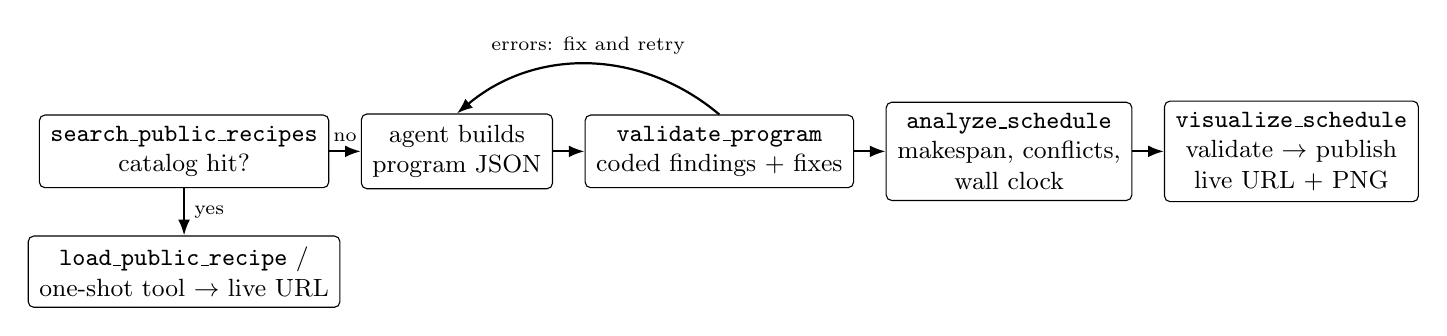
\begin{tikzpicture}[
    node distance=6mm and 4mm,
    box/.style={draw, rounded corners=2pt, minimum height=7mm, align=center, font=\small, inner sep=4pt},
    arr/.style={-{Latex[length=2mm]}, thick},
  ]
    \node[box] (search) {\code{search\_public\_recipes}\\catalog hit?};
    \node[box, right=of search] (build) {agent builds\\program JSON};
    \node[box, right=of build] (val) {\code{validate\_program}\\coded findings + fixes};
    \node[box, right=of val] (ana) {\code{analyze\_schedule}\\makespan, conflicts,\\wall clock};
    \node[box, right=of ana] (viz) {\code{visualize\_schedule}\\validate $\rightarrow$ publish\\live URL + PNG};
    \node[box, below=of search] (load) {\code{load\_public\_recipe} /\\one-shot tool $\rightarrow$ live URL};
    \draw[arr] (search) -- node[above,font=\scriptsize]{no} (build);
    \draw[arr] (search) -- node[right,font=\scriptsize]{yes} (load);
    \draw[arr] (build) -- (val);
    \draw[arr] (val) -- (ana);
    \draw[arr] (ana) -- (viz);
    \draw[arr] (val.north) to[out=140,in=40] node[above,font=\scriptsize]{errors: fix and retry} (build.north);
  \end{tikzpicture}}
  \caption{The workflow the server's \code{instructions} describe to the host at initialization. Catalog content is returned with its live URL directly; new content is validated before it can be published.}
  \label{fig:flow}
\end{figure}

\paragraph{Tools.} Each of the thirteen tools is registered with a title and MCP annotations (\code{readOnlyHint}, \code{destructiveHint}, \code{idempotentHint}, \code{openWorldHint}); four (validation, analysis, search and publication) also carry an output schema and return \code{structuredContent}, so that hosts which honour annotations can auto-approve read-only calls and agent frameworks can consume results without parsing markdown. The annotations are self-declared hints, and a host is free to ignore them. \code{validate\_program} and \code{analyze\_schedule} are pure and read-only. \code{visualize\_schedule} validates first and by default refuses an invalid program with the same coded findings (an explicit \code{allowInvalid} flag publishes a rough draft anyway), then creates a share record and returns a markdown preview (cover image, equipment, ingredients, an ASCII Gantt, the itinerary and a schedule check), an inline PNG of the timeline, and the live URL. \code{import\_from\_source} wraps the importer registry; \code{create\_environment} produces an environment document; \code{search\_public\_recipes} and \code{load\_public\_recipe} read the public catalog; \code{login}, \code{list\_my\_programs}, \code{load\_program} and \code{save\_program} handle a user's own library, with \code{save\_program} also validating first. Failures set \code{isError} and say what to do next, including when a call needs a login token.

\paragraph{Resources and prompts.} The server publishes the program JSON Schema, a one-page authoring guide (the rules the validator enforces, the trigger vocabulary, how to make tracks finish together, choice branching), and five complete example programs as MCP resources, and a \code{plan\_schedule} prompt that takes a goal, an optional deadline and optional resource limits and walks the model through the workflow in Figure~\ref{fig:flow}. Server-level \code{instructions} carry the workflow once per session rather than repeating it in every tool description.

\paragraph{Why this matters.} In our experience the failure mode of an LLM asked to ``plan Thanksgiving with one oven'' is a wall of prose that is wrong about timing and impossible to follow at the stove. Giving the model a validator with fix hints, an analyzer that answers ``when do I start,'' and a publisher that refuses malformed input by default moves the burden of \emph{structural} correctness (identifiers, dependencies, overlaps, declared resources) from the model's text to the tool contract, and the deliverable from a chat message to a page on the cook's phone. Whether the durations and orderings the model chooses are sensible is not something the validator can check. This is the LLM-Modulo arrangement, in which the model generates candidates and external, sound critics verify them rather than the model being trusted to plan~\cite{kambhampati2024llmmodulo}, a division the planning benchmarks motivate directly~\cite{valmeekam2023planbench}. The pattern is not unique to \rt{}: Benyamin et al.'s Planning Copilot exposes syntax checking, planner selection, plan validation and execution simulation to an LLM as MCP tools for the same reason~\cite{benyamin2025copilot}, and Angelopoulos et al.\ pair natural-language protocol authoring with automated validation for a lab orchestrator~\cite{angelopoulos2026prompts}. What \rt{} adds is the domain (a person's timeline rather than a planner's plan or a robot's protocol) and the publication step. We now report it as a measurement. Following Almuntashiri et al.'s protocol for extracting structured records from text~\cite{almuntashiri2025provenance}, and the question-refinement and cognitive-verifier prompt patterns catalogued by White et al.~\cite{white2023prompts}, we replaced the single \code{plan\_schedule} message with four turns---read-back, target-model check, extraction of steps with the source span each came from, the schema-constrained, span-attributed extraction Dagdelen et al.\ apply to scientific text~\cite{dagdelen2024extraction}, and only then relationships---and scored both against 24 expert-authored programs (10 kitchen, 6 laboratory, 4 event, 4 fitness), each paired with its source text and per-step spans. On \code{claude-haiku-4-5} the four turns raise relationship (trigger) F1 from 0.22 to 0.63 and the end-to-end pass rate---both validators pass, makespan within 10\% of the expert's, critical chain sharing at least half its steps---from 0.08 to 0.62. The gain is in extraction rather than in inference: asking for the step list before any dependency exists lifts step recall from 0.37 to 0.95 and cuts the unsupported (unattributable) step rate from 0.60 to 0.01, so the triggers have real steps to point at; relationships nevertheless remain the weakest component, as the paper also found. The gold set, the harness (\code{rhylthyme eval-prompts}) and the committed per-program numbers ship with the repository, so a prompt change is gated on them in CI.

\section{Discussion: positioning}
\label{sec:discussion}

Table~\ref{tab:position} summarizes the comparison. \rt{} \emph{borrows} the Gantt row-per-track grammar, the RCPSP resource model, the idea of a critical chain, and the trigger vocabulary of temporal constraint networks. It \emph{omits} what most of the compared systems are built around: it does not optimize an objective, does not reason about durations outside the executor's control, does not solve actor assignment, and does not execute anything on a machine. What is \emph{new} is narrower than a new model of human work: in the language and both runtimes the person is a capacity-one resource whose duration oracle is a button, and the human-specific constructs are the triggers that wait for that button, the attention fractions in environments, and the affordances of the runtimes. The claim is that no compared system combines capacity constraints and cross-track dependencies with a followable, human-executed timeline that has manual, executor-ended and abort steps; that the same schema is used unchanged across cooking, laboratory, event and training verticals, with domain content kept in metadata and environments rather than in the schema; and that validation, analysis and publication are exposed as typed, annotated tool calls rather than as instructions in a prompt. Table~\ref{tab:position} compares traditions rather than individual systems, so its cells describe the mainstream of each column, and specific systems (a workflow platform's MCP server, a lab orchestrator's guided manual steps) already occupy some of the cells the \rt{} column claims.

\begin{table}[t]
  \centering\scriptsize
  \setlength{\tabcolsep}{3.5pt}
  \begin{tabular}{@{}lR{2.1cm}R{2.1cm}R{2.1cm}R{2.3cm}R{2.2cm}R{2.4cm}@{}}
    \toprule
    Axis & CPM / PERT / RCPSP & ATC flow mgmt & Robot task scheduling & Lab automation orchestrators & Workflow engines & \textbf{\rt{}} \\
    \midrule
    Executor & human, offline & controllers, airlines, live & robots and human--robot teams & instruments, robots, guided manual steps & compute nodes & \textbf{a person, live} \\
    Author & analyst, PM & traffic manager & roboticist & automation engineer & bioinformatician & \textbf{domain expert or LLM agent} \\
    Temporal semantics & precedence + durations & slots, windows, replanned & STN/STNU, temporospatial & synchronization, stations & data-dependency DAG & \textbf{wall-clock triggers incl.\ manual, indefinite} \\
    Objective & makespan, NPV & delay cost under capacity & feasible or near-optimal & throughput under scientific constraints & reproducible, portable output & \textbf{followable timeline; feasibility, conflicts} \\
    Resources & renewable & sector, airport capacity & robot capabilities & stations & CPU, memory, containers & \textbf{maxConcurrent per task; actors (attention in the CLI runner)} \\
    Uncertainty & PERT beta, stochastic & stochastic demand & contingent durations & process variance & retries & \textbf{variable and indefinite, executor-ended} \\
    Portability & tool-specific & domain-specific & domain-specific & SiLA, Autoprotocol & containers, standards & \textbf{one schema, environments per workplace} \\
    Agent interface & none & none & none & emerging (vendor and community MCP servers) & emerging (vendor MCP servers) & \textbf{native MCP} \\
    \bottomrule
  \end{tabular}
  \caption{Positioning \rt{} against the traditions in Section~2. Cells describe the mainstream of each tradition, not every system in it.}
  \label{tab:position}
\end{table}

The nearest neighbours deserve a direct comparison. The cooking-step schedulers of Matsushima and Funabiki and of Nakabe et al.~\cite{matsushima2015cooking,nakabe2021cooking} and the SDL scheduler of Zhou et al.~\cite{zhou2026sdlscheduling} model the same objects (parallel procedures, shared stations, tight synchronization) and solve for an optimized procedure; \rt{} would be a natural \emph{target} for their output, since none produces a shareable runtime or an agent interface. Protocol run modes and guided-cooking timers are the other neighbour: they have the runtime but not the model, so a second dish or a second protocol cannot be placed against the first. The mixed-initiative scheduling workbenches~\cite{hsu1993macmerl,norbis1996interactive} had both a model and a human in the loop, but the human's role was to edit the schedule, not to execute it. Workflow engines and lab orchestrators, finally, would be natural \emph{consumers} of \rt{}'s trigger vocabulary if the executor were a machine; the language is agnostic about that, but the runtimes are not.

\section{Limitations and future work}
\label{sec:limits}

The auto-planner is a heuristic with no optimality guarantees. Variable and indefinite steps are ended by the executor, so a program's uncertainty is under the executor's control; the case the temporal-networks literature treats, a step whose end is decided by a process (an incubation, a rise), is not represented, and adding it would make dynamic-controllability checking~\cite{morris2001dc} the right tool for ``start twenty minutes before the roast is done.'' Today that construct is only partly honest: a negative offset has to fire before its anchor ends, so both runtimes resolve it against a \emph{projection} of that end rather than the end itself. The projection is the author's \code{defaultSeconds} unless the program opts in with \code{metadata.offsetsUse} set to \code{predicted}, in which case an indefinite anchor is projected from the program's own run history whenever a prediction exists whose interval is narrower than the authored default; an anchor that ends before the projected instant releases the trigger immediately, so a projection can delay work but never hold it back once the thing it was projecting has happened. A roast that finishes early or late is therefore compensated only to the extent that history predicts it in advance, and not at all once the run is under way. The two validators agree on timing but not on coverage: only the Python one applies the JSON Schema, and only the JavaScript one detects dependency cycles and unparseable durations; a single specification both implement is overdue. The web application's clock is a simulated player clock, not a wall-clock dispatcher. Actor constraints are accounted for but not solved; a small assignment layer along the lines of Tercio~\cite{gombolay2018tercio} is the obvious next step for multi-person kitchens and labs. When several people follow one program, each runs their own copy of the clock; merging progress across participants, the CDM idea, is not implemented, and the reactive rescheduling that the scheduling literature has treated as central since the 1990s~\cite{kelleher1997rescheduling} is limited to delay propagation. The rhythm of cues and manual gates is fixed by the program; the evidence that interaction timing shapes users' agency~\cite{yu2017timing} suggests it should be a design parameter. The reported critical chain is a heuristic and not a float-based critical path, and the web application's live page computes step timings with its own routine, which the parity test does not yet cover. Import quality is bounded by source structure, recipe text under-specifies durations, and the Opentrons importer executes fetched protocol code, which needs a proper sandbox before it should accept arbitrary URLs. Durations are no longer only author guesses, which matters because authored estimates are systematically optimistic: people underestimate how long their own tasks will take, and do so even when they have the relevant history~\cite{buehler1994planning,kahneman1979intuitive}. Learning durations from recorded executions instead is what the process-mining literature does for remaining flow time, from annotated transition systems over event logs to stochastic Petri nets with arbitrary firing delays~\cite{vanderaalst2011prediction,roggesolti2013remaining}. Badosa et al.\ predict each bioinformatics job's performance from its execution history under different combinations of cluster resources, and co-schedule jobs on one node only when they are compatible~\cite{badosa2019resource}. Both \rt{} runtimes now write one run record per execution --- the planned and the actual start and end of every step, what ended each non-fixed step, and the author-declared variance factors the executor answered at run start --- and the same identical-then-similar lookup runs over those records: an identical context yields a median and an interval, otherwise a per-step least-squares fit on the factors whose correlation with the observed duration clears a threshold. A held-out evaluation, which trains on a program's earlier runs and predicts its latest fifth, measures the result against the author's number. On a synthetic corpus with a known generating law it recovers that law: for an indefinite step whose duration is a function of a declared factor the mean absolute error falls from 2\,h\,26\,min, the authored \code{defaultSeconds}, to 81\,s, a 99\,\% reduction; for a step whose observed durations were generated around the authored value itself, prediction is 26\,\% \emph{worse}, because there the author's number is already the true mean and history can only add estimation noise to it. Which of the two a real step resembles is an empirical question per step, decided by the same variance analysis Badosa et al.\ use to establish that a history is inferential at all; the corresponding measurement on real catalog runs awaits a thirty-day observation window and is not reported here. What remains absent is the reactive half: prediction changes when a negative offset fires and which durations the planners are shown, but nothing is rescheduled while a run is in progress. Compatibility-based co-scheduling is the machine counterpart of the fractional \code{actorsRequired} model and is likewise not implemented. The MCP server's login is a pasted, short-lived bearer token that passes through the model's context, outside the protocol's OAuth framework; adopting it would remove that step and that exposure for consumer hosts. Three example programs fail both validators (two for within-track overlaps, one for undeclared resources), which is evidence both that the checks are useful and that authoring remains error-prone. Finally, the language has no formal semantics beyond the schema, its OWL-Time annotations and the reference validators; writing one down would make the controllability and assignment work well-posed.

\paragraph{Activity recognition: from timer to conductor.} Every runtime described here learns what the executor is doing only from what the executor tells it: a tap on a manual gate, a ``done'' on an indefinite step. The complementary technology is activity recognition, which infers from video, audio or wearable sensors which action a person is performing~\cite{kong2022survey}. It is furthest along in the operating room, where surgical phase and tool recognition from laparoscopic video is a mature line of work~\cite{twinanda2017endonet} and the surgical data science agenda explicitly asks for workflow-aware assistance that knows where in the procedure the team is~\cite{maierhein2017sds}; egocentric and multi-view datasets of kitchen and assembly work now provide the fine-grained action labels, procedural structure and mistake annotations that step-level recognition needs~\cite{damen2018epic,grauman2022ego4d,sener2022assembly101}. The bench laboratory is being treated the same way. ProBio is a multimodal dataset of molecular-biology lab work whose annotations are guided by the written protocol, with benchmarks for tracking transparent solutions and for action recognition that fuses video with the protocol text~\cite{cui2023probio}; FineBio records 32 participants performing mock experiments and annotates them as a hierarchy of protocol, steps and atomic operations, observing that biology requires strict adherence to the step order while leaving the order of operations within a step free, which is exactly the track-and-step structure of a \rt{} program~\cite{yagi2025finebio}; and a step-aware safety monitor built on protocol-annotated lab video first aligns the footage to the protocol to find the current step, then checks the step-specific constraints~\cite{xu2026labsafety}. Coupling a recognizer to a \rt{} program is a natural next step, and the coupling runs both ways. A recognizer that emits step-start and step-end events (the tube is capped, closure has begun, the actor has left the stage) would end indefinite steps and fire negative offsets from the observed end rather than from any projection, authored or predicted, removing the limitation noted above, and would make actor availability observable rather than declared. In the other direction the program is a strong prior: at any moment only a few steps can legitimately start, so the label space the recognizer must discriminate collapses from every action in the vocabulary to the handful the schedule allows, the ordering constraint that surgical phase models exploit and the reason ProBio and its successors condition recognition on the protocol. With both halves in place \rt{} would act as a conductor for a team rather than a timer for an individual: it would see every track at once, cue each technician, nurse or stagehand at the moment their step becomes ready, and replan the remaining tracks when someone runs long, in a bench laboratory with several people on one protocol, an operating room, or a theatre where cues follow the action on stage rather than a stopwatch. The obvious risks are that a recognizer which advances the clock wrongly is worse than a timer, and that cameras in these rooms raise privacy and consent questions; the mixed-initiative reading is that recognized transitions should be proposed and confirmed until their reliability is measured, which the runtimes' manual gates already support. None of this is implemented; it is the direction in which the \code{manual} and \code{indefinite} constructs, and the actor model, were designed to be extended.

\section{Conclusion}

\rt{} is a small, opinionated answer to a common situation: a person, a clock, several things happening at once, and not enough ovens. It reuses well-understood ideas from project scheduling and temporal reasoning, packages them in a schema that survives being moved between kitchens, laboratories, stages and gyms, plays the result live with the resource model still in force, and, through MCP, lets a language model do the authoring against a tool contract that refuses by default to publish what will not work.

\paragraph{Availability.} The specification, example programs and environments, the command-line runner, the timeline engine (\code{rhylthyme-timeline}) and the MCP server implementation (\code{rhylthyme-mcp}) are public at \url{https://github.com/rhylthyme}; the web application and importers are being prepared for release under the same organization. The remote server is at \url{https://mcp.rhylthyme.com/mcp}. This report describes the repositories as of September 2026 and is released under CC BY 4.0.

\bibliographystyle{plainnat}
\bibliography{references}

\end{document}
